\chapter{Results and Discussion}
Matrix Factorization are widely used in recommender systems for e-commerce. In this chapter follows a presentation of the results achieved in this project using our own implementation of The Latent factors algorithms applied to the a dataset from a live e-commerce system. This chapter will focus on the actual results. For evaluation and discussion regarding how good the results were, see Chapter 7.

\section{Recommendation Algorithm Evaluation}
Taking a privacy-preserving approach, recommendations performed by the implementation of the algorithms, the application is presented below. Graphs of each sub category is shown and subsequent comparison table is constructed.

\begin{table}[h]
\centering
\begin{tabular}{ llllll }
\toprule
\textbf{Method} & \textbf{Time for Training the Model} & \textbf{RMSE} & \textbf{Recall} & \textbf{Precision}  \\
\midrule
Matrix Factorization & 70.49s & 1.1914 & 0.473 & 0.798  \\
\hline
Topic Modelling & 65.33s & 1.8145 & 0.631 & 0.539 \\
\hline
Combined Model & 117.89s  & \textbf{1.0787} & 0.588 & 0.751 \\ 
\bottomrule
\end{tabular}
\caption{Digital Music Results}
\label{Digital Music Results}
\end{table}



\begin{table}[h]
\centering
\begin{tabular}{ llllll }
\toprule
\textbf{Method} & \textbf{Time for Training the Model} & \textbf{RMSE} & \textbf{Recall} & \textbf{Precision}  \\
\midrule
Matrix Factorization & 89.49s & 1.1957 & 0.398 & 0.738  \\
\hline
Topic Modelling & 105.45s & 1.714 & 0.588 & 0.550 \\
\hline
Combined Model & 125.45s  & \textbf{1.1134} & 0.671 & 0.686 \\ 
\bottomrule        
\end{tabular}
\caption{Health and Personal Care Results}
% \label{Health and Personal Care Results}
\end{table}


\begin{table}[h]
\centering
\begin{tabular}{ llllll }
\toprule
\textbf{Method} & \textbf{Time for Training the Model} & \textbf{RMSE} & \textbf{Recall} & \textbf{Precision}  \\
\midrule
Matrix Factorization & 78.69s & 1.2914 & 0.510 & 0.780 \\
\hline
Topic Modelling & 97.45s & 1.6145 & 0.653 & 0.578 \\
\hline
Combined Model & 122.48s  & \textbf{1.1234} & 0.563 & 0.647 \\
\bottomrule        
\end{tabular}
\caption{Cell Phones and Accessories Results}\label{Cell Phones and Accessories Results}
\end{table}


In the above table we can see that the RMS values of the matrix factorization and topic modelling are quite good.
Then the experiment was conducted with two models combined and as we can see that RMSE value of combined models is 1.0787.

% \vfill
Below, we can observe the results and topics generated by the LDA algorithm,

\begin{figure}[H]
  {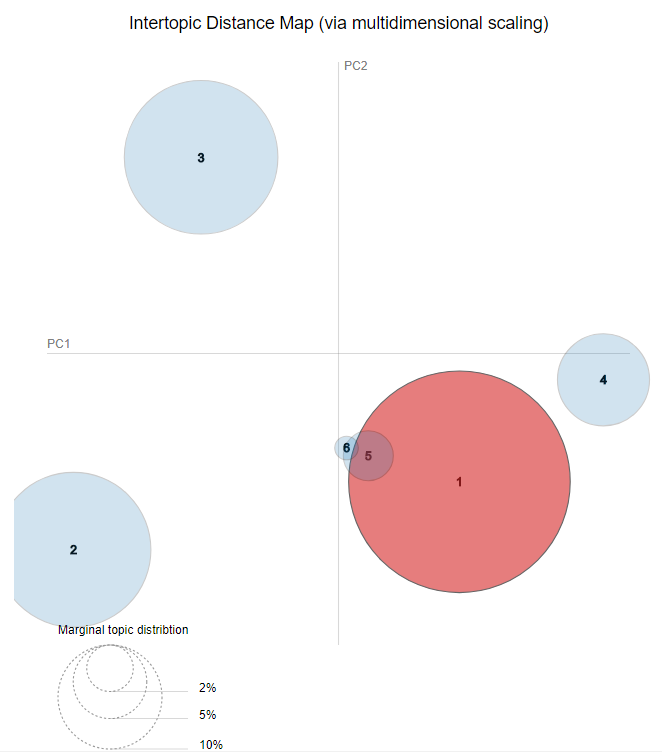
\includegraphics[width = 0.85 \textwidth]{img/lda/1.PNG}}
  \caption{Principal Component Analysis for Topic Modelling Digital Music Dataset}
\end{figure}

\begin{table}[h]
\centering
\begin{tabular}{ llllll }
% \toprule
%  &  &  &  &  \\
\midrule
music  & live  & like  & quot  & quot & mixer \\
album  & james  & cd  & live  & mr  & bass \\
soul   & time  & live  & jb  & brown  & synth \\ 
like  & best  & just  & studio  & james & jbl \\ 
great  & band  & band  & loose  & machine & flute \\ 
right  & brown & bootsy  & world & band & crowd \\ 
brown   & funk  & doing  &  time  &  good & drum \\ 
just   & album  & sex & great &  funk  & tempo \\ 
\bottomrule          
\end{tabular}
\caption{Music Labels}
\label{Music Labels}
\end{table}



\begin{figure}[H]
  {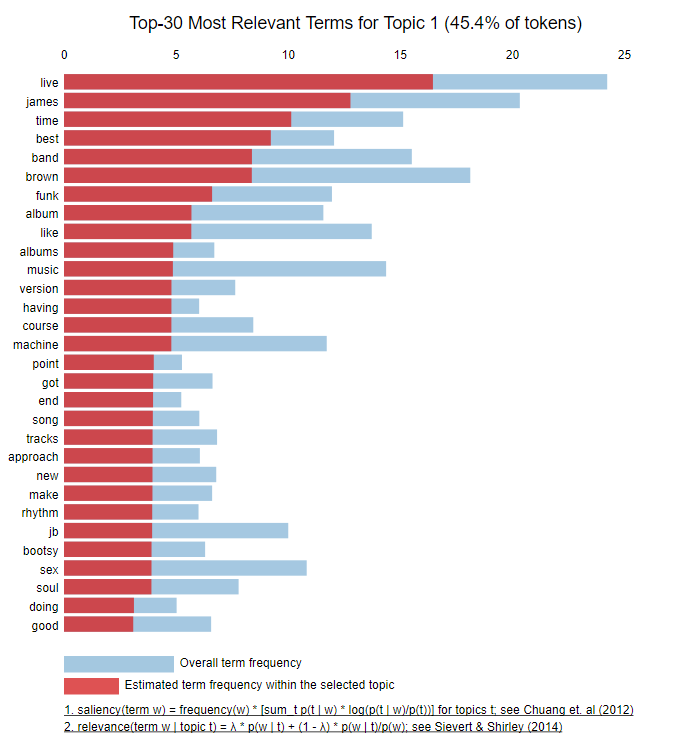
\includegraphics[width = 0.85 \textwidth]{img/lda/1a.PNG}}
  \caption{Topic Distribution on Digital Music Dataset}
\end{figure}


% \begin{table}[h]
% \centering
% \begin{tabular}{ lllll }
% \toprule
%  &  &  &  &  \\
% \midrule
% music  & live  & like  & quot  & quot  \\
% album  & james  & cd  & live  & mr  \\
% soul   & time  & live  & jb  & brown  \\ 
% like  & best  & just  & studio  & james  \\ 
% great    & band  & band  & loose  & machine \\ 
% right  & brown & bootsy  & world & band  \\ 
% brown   & funk  & doing  &  time  &  sex \\ 
% just   & album  & sex & great &  funk \\ 
% \bottomrule          
% \end{tabular}
% \caption{Labels Table}
% \label{Labels Table}
% \end{table}


\begin{figure}[H]
  {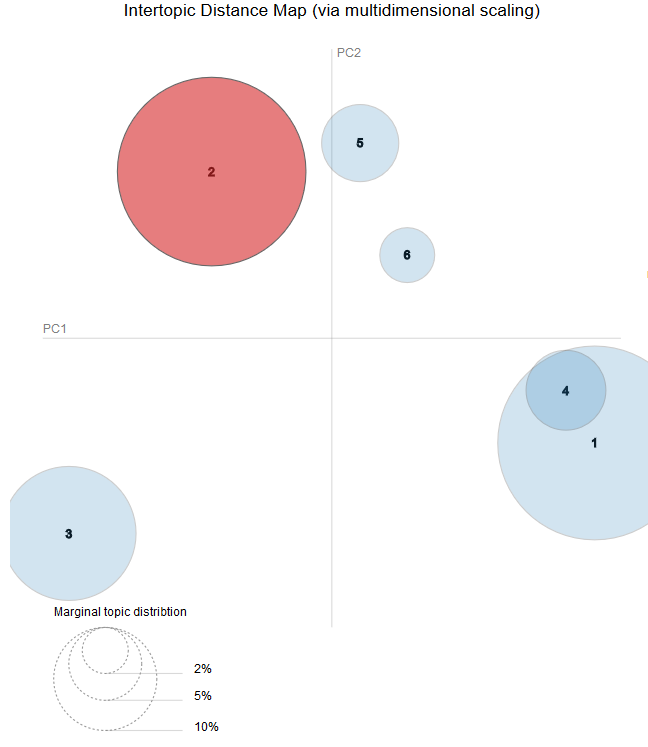
\includegraphics[width = 0.85 \textwidth]{img/lda/2.PNG}}
  \caption{Principal Component Analysis for Topic Modelling Health and Personal Care Dataset}
\end{figure}



\begin{table}[h]
\centering
\begin{tabular}{ llllll }
% \toprule
%   &  &  &  &  &  \\
\midrule
computer & fitbit & fitbit & day & walk & calories \\
calories & app & far & track & weight & fitbit \\
eat & sleep & lost & fitbit & just & active \\
burned & just & device & easy & device & app \\
weight & really & good & computer & read & steps \\
good & great & track & sleep & sleep & don \\
steps & need & read & great & help & burned \\
tells & does & kindle & like & stairs & help \\
\bottomrule          
\end{tabular}
\caption{Health and Personal Care Labels}
\label{Health and Personal Care Labels}
\end{table}

\begin{figure}[H]
  {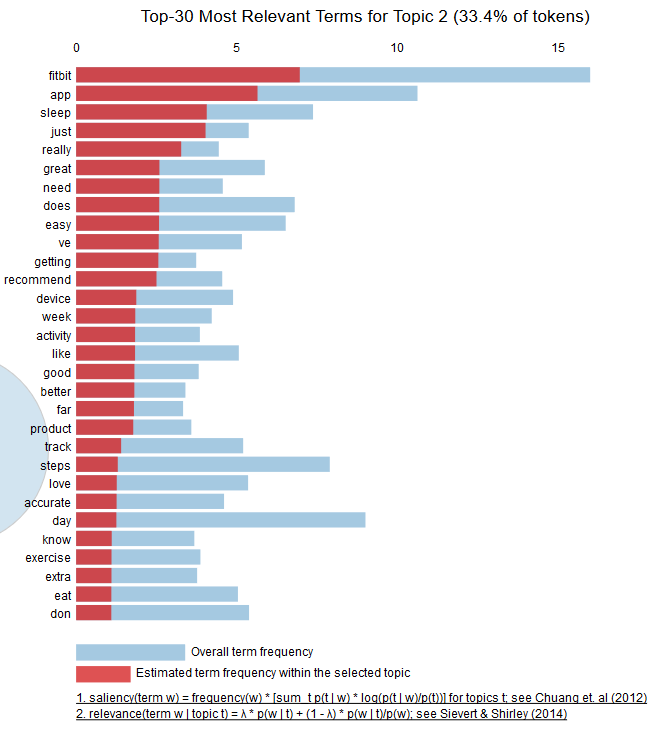
\includegraphics[width = 0.85 \textwidth]{img/lda/2a.PNG}}
  \caption{Topic Distribution on Health and Personal Care Dataset}
\end{figure}

\begin{figure}[H]
  {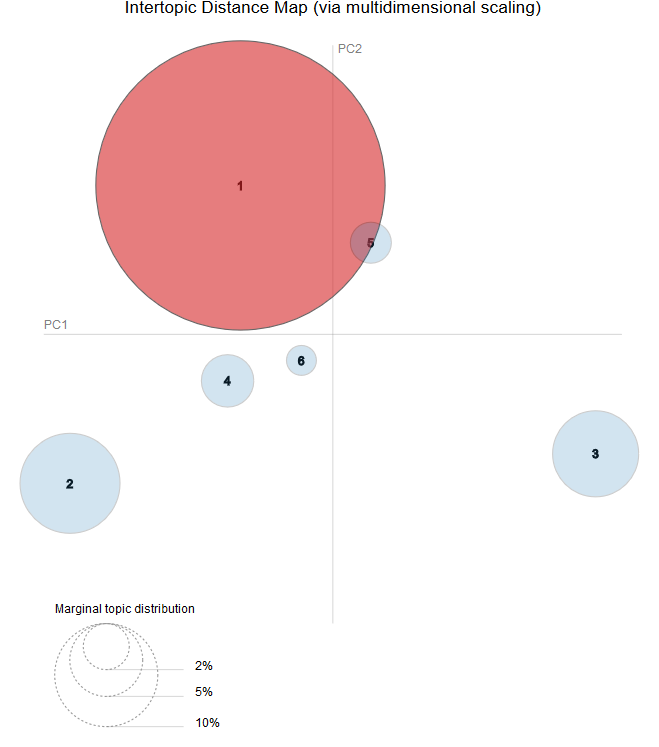
\includegraphics[width = 0.85 \textwidth]{img/lda/3.PNG}}
  \caption{Principal Component Analysis for Topic Modelling CellPhones and Accessories Dataset}
\end{figure}


\begin{table}[h]
\centering
\begin{tabular}{ llllll }
% \toprule
%  &  &  &  &  \\
\midrule
battery & batteries & red & works  & quot & cable \\
charger & battery & charging & batteries  & mr & amplifier \\
charge & just & blue & charges & brown & plug \\ 
phone & phone & charger & product & james & power \\ 
batteries  & spare & use  & great & machine & backup \\ 
usb & brown & light & different  & band & output \\ 
charging & like & works & charged & drum & speaker \\ 
use & port & brilliant & just &  thing & earphones \\ 
\bottomrule          
\end{tabular}
\caption{Cell Phones and Accessories Labels}
\label{Cell Phones and Accessories Labels}
\end{table}

\begin{figure}[H]
  {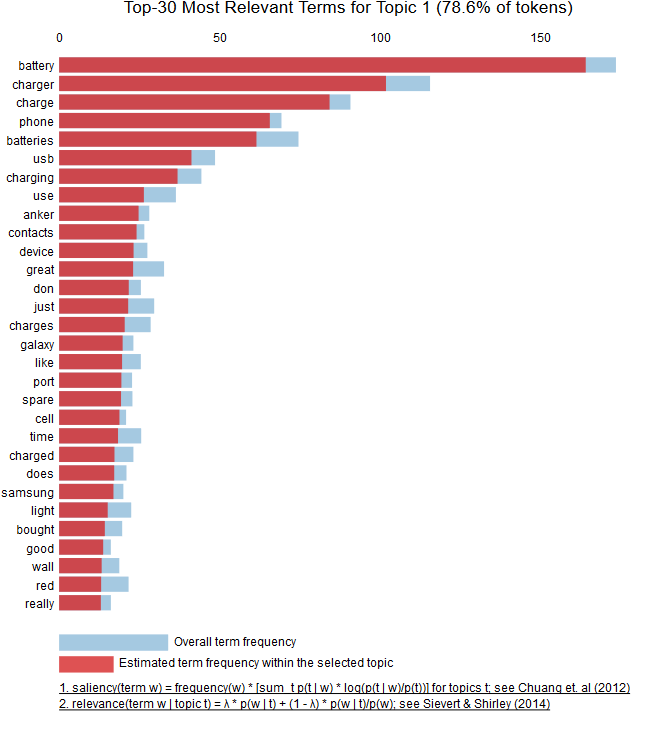
\includegraphics[width = 0.85 \textwidth]{img/lda/3a.PNG}}
  \caption{Topic Distribution on CellPhones and Accessories Dataset}
\end{figure}


This shows a significant increase in the model accuracy, consequently this type of approach can be used to improve the recommendations generated by the system.

\begin{itemize}
    \item Always recommend items based on gender. (Men and women always buy the same items as other men and women, respectively)
    \item Always recommend items based on age. (People at a certain age always buy same items as other people in the same age)
    \item Always recommend items based on domicile. (People from city X always buy the same items as other people from city X)
    \item Baselines have been used before any other extensive evaluation method, something that has been of great help when implementing the application, as these baselines can be seen as evaluation in its most basic form.
\end{itemize}


